\section{Training}

A preprocessor was used that resampled the fundamental frequency and loudness, taking account the sample rate, frame rate, and number of timesteps. The number of timesteps was set at 1000 per 4 second clip, giving a spectral resoluiton of 4ms per timestep. This was deemed to be the best compromise between computational efficiency and accuracy.

An autoencoder encoder decoder setup was used. The encoder was based on Mfcc variant of a \acrfull{RNN}. The decoder was a RNN based decoder as described previously in \nameref{sec:singing_voice_synthesis}.

The model settings were kept the same as in \nameref{sec:singing_voice_synthesis} as they had already validated their hyperparameter selection. This included the use of100 sinusoidal harmonic components and 60 filter banks. This was done to limit model size to ensure it fitted on one GPU.

Each model was trained for 200,000 epochs, training time was approximately 2.9 epochs per second or 5.2 epochs per second depending on GPU used. Total training time was approxumately 20 horus per model.

\begin{figure}
    \centering
    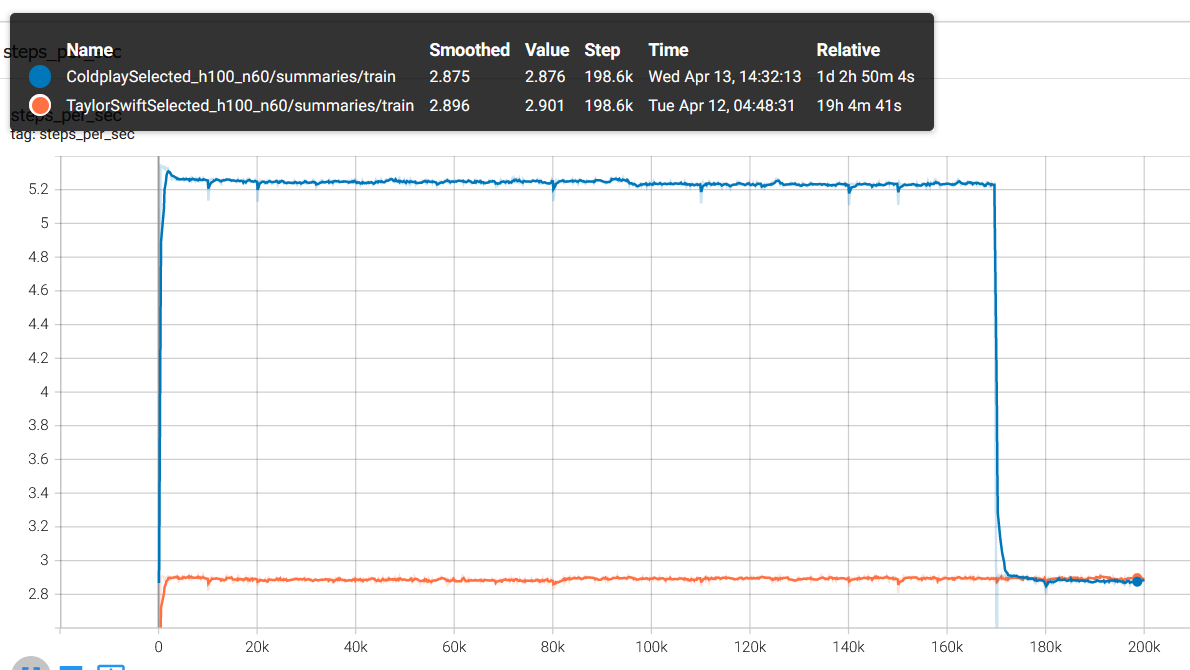
\includegraphics[width=0.6\textwidth]{research/training/StepsPerSecond.png}
    \caption{Training steps per second over the 200,000 training epochs}
\end{figure}

\begin{figure}
    \centering
    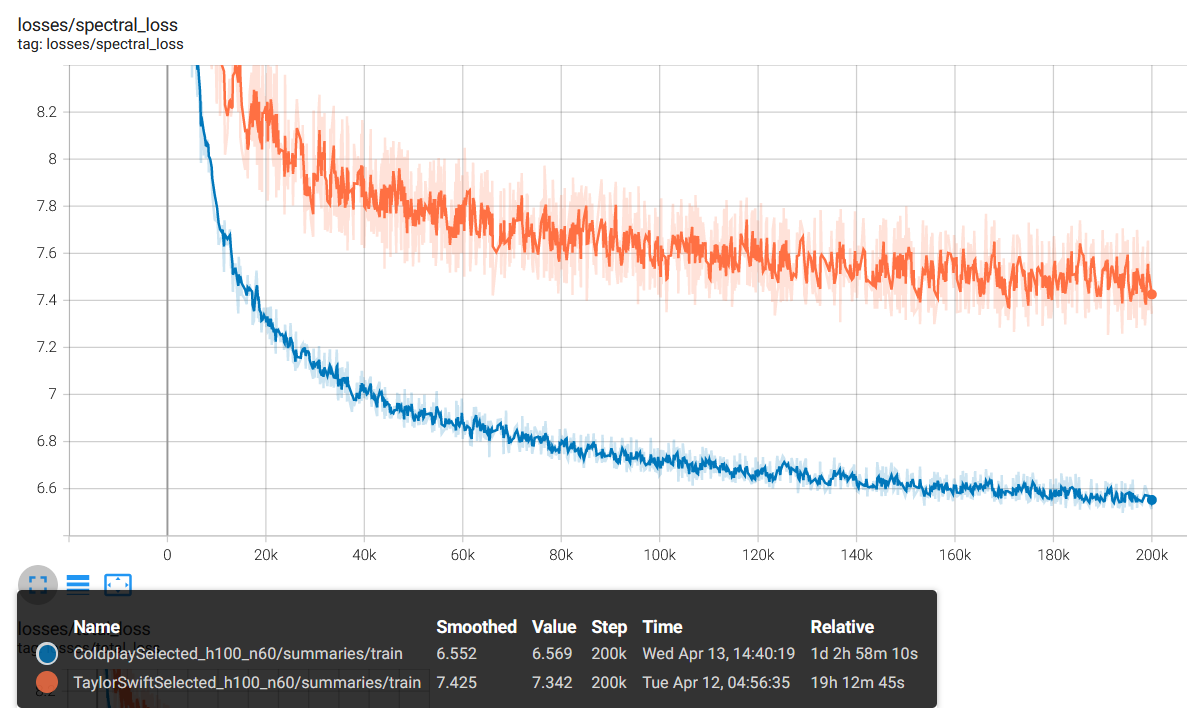
\includegraphics[width=0.8\textwidth]{research/training/TrainingSpectralLosses.png}
    \caption{Training Spectral Losses: Losses over the 200,000 epochs of training both models, using the spectral loss function defined in \nameref{sec:loss_measure}}
    \label{fig:training_spectral_losses}
\end{figure}

\nameref{fig:training_spectral_losses} shows the Coldplay losses being less than the Taylor Swift losses. This is due to the fact that the Coldplay Dataset having more frames that were pure silence, meaning that the Coldplay model fitted the silence frames more accurately.

